\documentclass[11pt,a4paper]{jarticle}
\usepackage[dvipdfmx]{graphicx}
\usepackage{url}

\renewcommand{\baselinestretch}{1.05} 
\marginparwidth=0cm
\topmargin=-1cm
\headheight=0.3cm
\headsep=0.7cm
\oddsidemargin=0cm
\evensidemargin=0cm
%\textwidth=43zw
\textwidth=15.92cm
%\textheight=43.3\baselineskip
\baselineskip = 0.5744cm
\textheight=43\baselineskip

\itemsep=0.05\baselineskip
\parsep=0pt
\topsep=0.01\baselineskip
\partopsep=0pt
\listparindent=0zw

%% header and footer
\usepackage{fancyhdr}
\pagestyle{fancy}
\lhead{2014年度 春学期授業}
\chead{インタラクティブ・アート実習}
\rhead{担当教員: 松下 光範}
\cfoot{\thepage}
\renewcommand{\headrulewidth}{0pt}
\renewcommand{\footrulewidth}{0pt}

\usepackage{ascmac}
\usepackage{listings,jlisting}
\usepackage{color}
\definecolor{OliveGreen}{cmyk}{0.64,0,0.95,0.40}
\definecolor{colFunc}{rgb}{1,0.07,0.54}
\definecolor{CadetBlue}{cmyk}{0.62,0.57,0.23,0}
\definecolor{Brown}{cmyk}{0,0.81,1,0.60}
\definecolor{colID}{rgb}{0.63,0.44,0}
\definecolor{rulesepcolor}{gray}{0.666}
\lstset{
  language=Java,%プログラミング言語によって変える。
  basicstyle={\ttfamily\small},
  keywordstyle={\color{OliveGreen}},
  %[2][3]はプログラミング言語によってあったり、なかったり
  keywordstyle={[2]\color{colFunc}},
  keywordstyle={[3]\color{CadetBlue}},%
  commentstyle={\color{Brown}},
  %identifierstyle={\color{colID}},
  stringstyle=\color{blue},
  tabsize=2,
  %frame=trBL,
  %numbers=left,
  numberstyle={\ttfamily\small},
  breaklines=true,%折り返し
  %backgroundcolor={\color[gray]{.95}},
  framexleftmargin=0mm,
  frame=single,
  rulesepcolor=\color{rulesepcolor},
  captionpos=b
}


%%%%%%%%%%%%%%%%%%%%%%%%%%%%%%%%%%%%%%%%%%%%%%%%%%%%%%%%%%%%%%%%
\begin{document}
% title
\section*{\LARGE{第4講 Analog Output を用いて LED を制御する}}
%%%%%%%%%%%%%%%%%%%%%%%%%%%%%%%%%%%%%%%%%%%%%%%%%%%%%%%%%%%%%%%%

\section{Analog Output}

\section{LED を徐々に光らせる}
Analog Output を用いる LED を細かく制御することができます。

\subsection*{プログラム}
\begin{lstlisting}
import processing.serial.*;
import cc.arduino.*;
 
Arduino arduino;
int ledPin = 9;   // LEDが接続されたピン番号

void setup() {
  size(255, 255);
  arduino = new Arduino(this, Arduino.list()[6], 57600);
  arduino.pinMode(ledPin, Arduino.OUTPUT);   // LEDのピンの出力に設定
}

void draw() {
  arduino.analogWrite(ledPin, mouseX);   // マウスのx座標をLEDの明るさにする
}
\end{lstlisting}

\subsection*{回路}
\begin{figure}[h!]
 \centering
 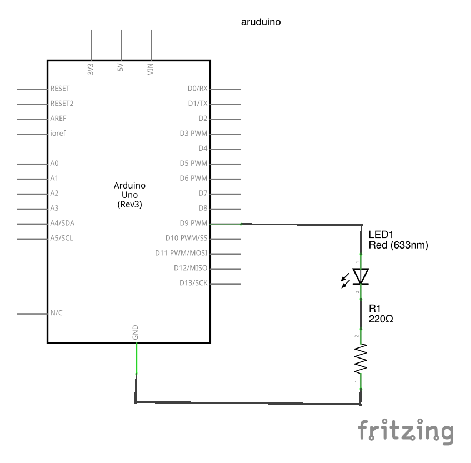
\includegraphics[width=0.5\columnwidth]{img/LED_circuit.eps}
 \caption{LEDのフェードインとフェードアウトの回路図}
\end{figure}

\section{フルカラー LED}
フルカラー LED を用いると、光の三原色をそれぞれ制御することによって、様々の色の表現が可能となります。
フルカラー LED の構造は単純で、内部に赤、緑、青の3つのLEDが入っていると考えれば良いです。
そのため、単色 LED のときは光り方を制御するために 1 つの Output を用いましたが、
フルカラー LED の場合は 3 色をそれぞれ制御する必要があるため 3 つの Analog Output を用います。
また、端子が 4 本出ているものが多いですが、これはアノード(+)またはカソード(-)が3つ分共通になっているためで、それぞれアノードコモン、カソードコモンと呼びます。

\begin{figure}[h!]
 \begin{minipage}{0.35\columnwidth}
  \centering
  \includegraphics[height=40mm]{img/full_color_led_detail.eps}
  \caption{フルカラー LED}
 \end{minipage}
 \begin{minipage}{0.65\columnwidth}
  本実習では、カソードコモンのものを用いる。% 要確認
  それぞれの端子は
  \begin{itemize}
   \item[R:] 赤
   \item[G:] 緑
   \item[B:] 青
   \item[K:] - (カソード)
  \end{itemize}
  に対応する。
  順番に注意すること!
 \end{minipage}
\end{figure}

\subsection*{プログラム}
\begin{lstlisting}
import processing.serial.*;
import cc.arduino.*;
 
Arduino arduino;
int LED_R = 9;    // LED 赤
int LED_B = 10;   // LED 青
int LED_G = 11;   // LED 緑

void setup() {
  size(255, 255);
  arduino = new Arduino(this, Arduino.list()[6], 57600);
  //LEDのピンを出力に設定する
  arduino.pinMode(LED_R, Arduino.OUTPUT);
  arduino.pinMode(LED_B, Arduino.OUTPUT);
  arduino.pinMode(LED_G, Arduino.OUTPUT);
}

void draw() {
  // LEDの明るさをセット
  arduino.analogWrite(LED_R, mouseX);
  arduino.analogWrite(LED_B, mouseY);
  arduino.analogWrite(LED_G, 127);
}
\end{lstlisting}

\subsection*{回路}
\begin{figure}[h!]
 \begin{minipage}{0.5\columnwidth}
  \centering
  \includegraphics[height=60mm]{img/Full_color_LED.eps}
  \caption{フルカラーLEDの配線図}
  \label{circuit}
 \end{minipage}
 \begin{minipage}{0.5\columnwidth}
  \centering
  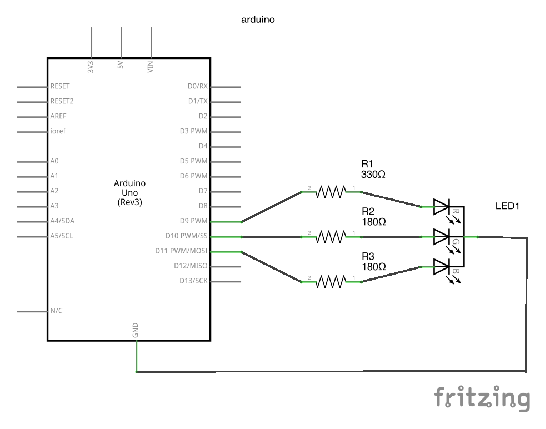
\includegraphics[height=60mm]{img/Full_color_LED_circuit.eps}
  \caption{フルカラーLEDの回路図}
 \end{minipage}
\end{figure}

\end{document}